\chapter{Array signal processing}
\label{ch:lit-rev}
This chapter presents an overview of beamforming using sensor
arrays. The first part of the chapter introduces the sensor array and
the conventional beamforming. The second part of the chapter
introduces the adaptive beamforming approach and defines the relevant
performance metrics used to evaluate the beamformers. The final
section describes the array polynomial representation of
beamformers. A more detailed treatment of the background topics can be
found in classic references \cite{vtree2002oap,johnson1992array}.

\section{Sensor array}
\label{sec:sensor_array} 
A sensor array is a collection of sensor elements arranged in a
defined geometry. Sensor arrays are used to measure spatially
propagating signals. Propagating signals could be electromagnetic,
acoustic or geophysical in nature depending upon the application
area. A propagating signal is a continuous space-time phenomena. The
sensor array samples the propagating signal at spatially discrete
locations to generate discrete samples. This spatial sampling is
analogous to the time sampling of continuous time (CT) signals to
generate discrete sequence \cite{Oppenheim1989}. Array signal
processing techniques process the sensor array measurements to filter
the propagating signals in space \cite{johnson1992array, vtree2002oap}.

% The sensor array measurement is
% represented as an $N \times 1$ vector
% \begin{align}
%   \label{eq:array-measure-vec-time}
%   \sigvec(t, \pos) = [\sig(t, \pos_0),~ \sig(t, \pos_1),~ \ldots,~ \sig(t, \pos_{N-1})]^T,
% \end{align}
% where $[\cdot]\trans$ is the vector transpose. A common operation on
% array measurement processes each sensor output by an LTI filter and
% sums the output to obtain array output
% \begin{align}
%   \label{eq:array-output-time}
%   \yt(t) = \sum\limits_{n = 0}^{N - 1} \hresp_n(t)*\sig_n(t, \pos_n),
% \end{align}
% where $\hresp_n(t)$ is the impulse response of the LTI filter applied to the
% $n$th sensor output. 

Consider an array of $N$ isotropic sensors at spatial locations
$\pos_n$ where $n = 0,\ldots, N-1$.  Let $\sig(t)$ be the signal at
the origin of the coordinate. As the signal wavefront propagates
across the array aperture, the observation at each sensor is a time
delayed version of $\sig(t)$. The delay occurs due to the finite
propagation time required for the signal to traverse the space from
the origin to sensor location. The array measured signal is
represented as a $N \times 1$ vector
\begin{align}
  \label{eq:array-measure-planewave-time}
  \sigvec(t, \pos) = [\sig(t - \tau_0), \sig(t - \tau_1), \ldots, \sig(t - \tau_{N-1})]^T,
\end{align}
where $\tau_n$ is the propagation time delay at the $n$th sensor. One
common operation processes the measurement from each sensor using a
delay filter with impulse response $\hresp_n = (1/N)\delta(t + T_n)$
such that the signals align in time. The time aligned signals are
summed to generate the output $\yt(t)$. If the filter delays are
chosen $T_n = \tau_n$, the filter processed signals are perfectly
aligned in time and add constructively producing output equal to the
original signal $\yt(t) = \sig(t)$. Thus the sensor array measurements
can be used to spatially filter the signals originating from a source
at a particular location if the delays $\tau_n$ are known. This
processor which delays and sums the sensor measurements is called the
delay-and-sum beamformer or the conventional beamformer (CBF).

% In frequency domain,
% $\yw(\omega) = \hrespWvec\trans(\omega)\sigWvec(\omega)$ where
% $\hrespWvec(\omega)$ is the vector of frequency response of the LTI
% filters and $\sigWvec(\omega)$ is the vector of Fourier transforms of
% signals measured at each sensor.

This dissertation focuses on the case of temporally narrowband
propagating signals. In the narrowband case, the delays ($\tau_n$) in the
array measurement \eqref{eq:array-measure-planewave-time} are
approximated by phase shifts \cite[Sec.~2.2]{vtree2002oap}. Hence, the
narrowband delay-and-sum beamformer can be implemented by applying
phase shifts to each sensor measurement and summing together. In general,
the beamforming operation combines the sensor measurements with some
complex weights $w_n$ to enhance or reject signals according to their
spatial dependence. The complex weight $w_n$ defines the gain and the
phase shift applied on the $n\nth$ sensor output. Defining the
beamformer weight vector as $\wt = [w_0, w_1, w_2\ldots w_{N-1}]^{T}$,
the beamformer output is $ y = \wt^H\sigvec$.

In many practical applications the sensor array is located in a
far-field region of the signal source. In the far-field region, the
signal propagation direction is approximately same at each sensor and
the signal wavefronts are approximated as planewaves
\cite{johnson1992array}. As the planewave propagates across the array
aperture the signal time delay ($\tau_n$) at each sensor depends on
the sensor location ($\pos_n$), propagation speed ($c$), and the
propagation direction ($\theta_0$). \sect{}\ref{sec:beamforming} discusses beamforming for planewave signals.

% Under the planewave assumption, the $n$th component of
% $\sigWvec(\omega)$ is
% \begin{align}
%   \label{eq:4}
%   \sigW_n(\omega) = \int\limits_{-\infty}^{\infty}\sig_n(t - \tau_n)\expo{-j\omega t}\, dt = \expo{-j\omega \tau_n}\sigW(\omega)
% \end{align}
% where $\omega\tau_n = \wavenum^T\pos_n$. Defining the vector
% \[ \rep(\wavenum) = [\expo{-j\wavenum^T\pos_0},
%   \expo{-j\wavenum^T\pos_1}, \ldots,
%   \expo{-j\wavenum^T\pos_{N-1}}]\trans, \]
% the measurement signal Fourier transform vector $\sigWvec(\omega) = \sigW(\omega)\rep_k(\wavenum)$. The vector
% $\rep(\wavenum)$ is called the array mainfold vector and it incorporates the  geometry and the spatial characteristic of the sensor array.

\section{Uniform linear array}
\label{sec:ula}
A uniform linear array (ULA) places the sensors on a straight line at equal
spacing. \figurename{}~\ref{fig:ula-geom} shows a schematic of a ULA
with $N$ sensors at uniform spacing equal to $d$. The sensors are
located at $p_n = nd$ for $\quad n = 0, 1, \ldots, (N - 1)$. For a ULA
designed to measure narrowband planewave signals, the standard choice
for sensor spacing is $d = \lambda/2$ where $\lambda$ is the wavelength
of the narrowband planewave signal of interest. The spatial sampling
interval of $\lambda/2$ is analogous to the Nyquist rate sampling of
CT signals with the sampling interval of $T/2$, where $T$ is the CT
signal period \cite{Oppenheim1989}. The remaining portion of the dissertation
focuses on beamforming for  narrowband planewave signals using a ULA with $d = \lambda/2$ sensor spacing.
\begin{figure}[!hp]
 \centering
    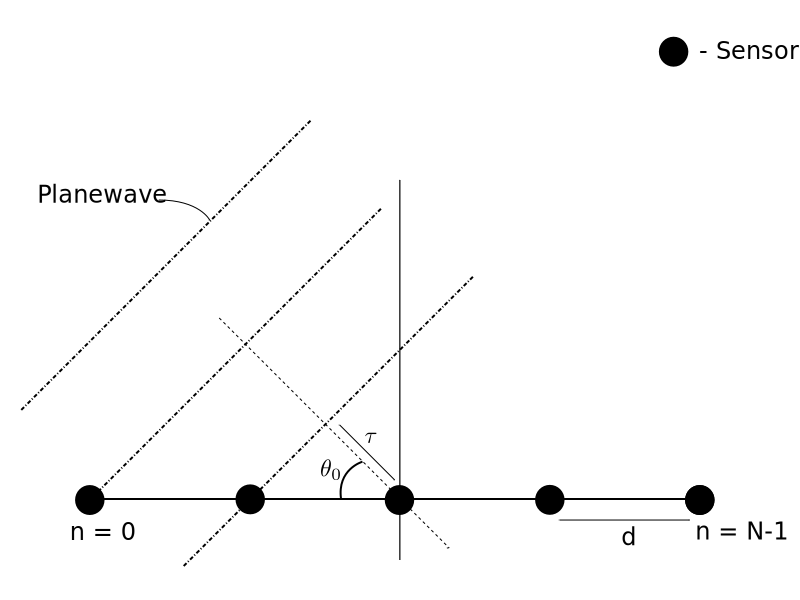
\includegraphics[width=\textwidth]{ula_planewave.pdf}
    \caption[Planewaves propagating across uniform linear array (ULA)]{Planewaves propagating across uniform linear array (ULA). The ULA has $N$ sensors (solid black circles) uniformly located at $d$ interval. The dashed arrow indicates planewave propagation direction which is expressed as angle $\theta_0$ w.r.t. the array axis. The direction along the array axis ($\theta = 0$) is called endfire and the direction perpendicular to the array axis ($\theta = \pi/2$) is called the broadside direction. The propagation time between two adjacent sensor is denoted by $\tau$.} 
 % Detailed descriptionof array geometry, broadside, endfire, bearing, axis, aperture
\label{fig:ula-geom}
\end{figure}

% The linear geometry of the ULA limits the direction resolution
% capability to elevation angles ($\theta$)
% \cite[Sec.~3.1.1]{johnson1992array}. In case of planewaves measured
% using ULAs, it is sufficient to define the propagation direction in
% terms of elevation angle. \figurename{}~\ref{fig:ula-geom} shows
% planewaves with propagation direction at an angle $\theta_0$ with
% respect to array axis. The direction along the array axis is called
% endfire ($\theta = 0$) and the direction perpendicular to the array
% axis is called broadside ($\theta = \pi/2$). Define the directional cosine
% $u = \cos(\theta)$. In the sequel, the planewave signal direction is
% denoted using directional cosine ($u$).

% Need to describe about the planewave in the figure
\figurename{}~\ref{fig:ula-geom} also shows narrowband planewaves
propagating across the ULA aperture. The dashed arrow indicates the
planewave propagation direction which is represented as angle
$\theta_0$ w.r.t. the array axis. The propagation direction along the
array axis is called endfire ($\theta = 0$) and the propagation
direction perpendicular to the array axis is called broadside
($\theta = \pi/2$). As the planewave propagates across the ULA
aperture from left to right, the planewave arrives at each sensor with
some time delay. Due to the uniform spacing of the sensors, the time
delay between adjacent sensors across the ULA is a constant
$\delay = d\cos(\theta_0)/c$ where $c$ is the speed of propagation. As
mentioned earlier, in case of narrowband planewave signals, the time
delay ($\delay$) is approximated by a phase shift
$\psi = (2\pi/\lambda)d\cos(\theta_0) = (2\pi/\lambda)d\ulook$ where
$\ulook = \cos(\theta_0)$ is the directional cosine. In the sequel, the
propagation direction of a planewave is expressed using the
directional cosine ($u$). Denoting the phase shifts at each sensor
w.r.t. a reference sensor at $p_0 = 0$ as a vector of complex
exponentials,
\begin{equation}
\label{eq:array-manifold}
  \rep(\ulook) = [1,~e^{-j{(2\pi d/\lambda)}  u_0},~ e^{-j{(2\pi d/\lambda)}2 u_0},
\ldots, e^{-j{(2\pi d/\lambda)}(N-1)  u_0}]^\text{T}.
\end{equation}
This vector of complex exponentials is referred to as the array
manifold vector \cite{vtree2002oap}. The array manifold vector
$\rep_0$ models the geometry and the spatial characteristic a ULA
observing a narrowband planewave signal with propagation direction
$\ulook$. The array manifold vector in \eqref{eq:array-manifold} is
defined such that $\norm{\rep(\ulook)}^2 = N$.

\subsection{Frequency domain snapshot model}
\label{sec:freq-snapshot}
In many cases, the beamforming operation is implemented in the frequency
domain \cite[Sec.~5.2.1]{vtree2002oap}. In the frequency domain, the ULA
measurement is expressed as a complex vector called frequency domain
snapshots. In order to generate the frequency domain snapshots, the
ULA observes the planewave signal for an interval $T$ during which the
source is assumed to be spatially stationary. The total observation
interval $T$ is divided into $L$ interval blocks of length
$\deltaT$. The following step performs an FFT on the signal observed
at each sensor for each interval block of length $\deltaT$. At each sensor, extracting the
complex coefficient from the FFT output associated to the narrowband
center frequency $f_0$ gives one snapshot vector. Let $X_n$ be the
complex coefficient associated with the $n^{th}$ sensor. The
narrowband planewave frequency domain snapshot vector is represented
as an $N \times 1$ complex vector $\x = [X_1,X_2,\ldots X_N]^T$. For a
single narrowband planewave signal propagating with directional cosine
$\ulook$, the frequency domain snapshot measured using the ULA is
modeled as $\x = a\rep_0$ where $a$ is the complex amplitude of
the planewave signal and $\rep_0 = \rep(\ulook)$ is the array manifold vector
corresponding to the planewave direction $\ulook = \cos(\theta_0)$.

% In the sequel, the frequency domain snapshot of narrowband planewave signals measured using a ULA is referred to as snapshot

\section{Planewave beamforming using a ULA}
\label{sec:beamforming} 
This section introduces beamforming with focus on narrowband planewave
signals observed using a ULA. Beamforming combines the entries of the
snapshot vector with complex weights to enhance the planewaves
arriving from a specific look direction and suppressing interfering
planewaves and noise. This operation is essentially spatial filtering
of planewave signals analogous to band pass filtering of time domain
signals where signals in a specific frequency band are allowed to pass
though while signals outside the band are suppressed. \figurename{}~\ref{fig:beamformer} illustrates the
beamforming operation on snapshot data obtained from a ULA. The beamformer applies a complex weight $w_n$ to
each entry of the ULA snapshot vector and sums to produce a scalar
output $ y = \wt^H\datavec$, where $\wt = [w_0, w_1, w_2\ldots w_{N-1}]^{T}$ is the beamformer weight vector.

\begin{figure} \centering
    \includegraphics[width=0.7\linewidth]{beamforming}
    \caption[Beamforming operation flow diagram]{Beamforming operation combines the frequency domain snapshot data with complex weights ($w_n$) to produce scalar output $\yt$.}
    \label{fig:beamformer}
\end{figure}

The CBF is the simplest beamformer applicable to ULA snapshot
data. The CBF weight vector phase shifts the snapshot entries such
that planewave signals from the look direction $\ulook$ align in time
and combine constructively while other signals combine destructively
and are suppressed. Hence, a CBF steered to the look direction
$\ulook = \cos(\theta_0)$ has a weight vector equal to the array
manifold vector associated with the look direction, i.e.,
$\wcbf = \rep_0/N$.

The beamformer weights are analogous to FIR filter coefficients. As
the choice of the filter coefficients determines the frequency
response of the FIR filter, the choice of the weight vector determines
the spatial response of a beamformer for a given ULA. The beampattern
defines the complex gain due to the beamformer for a unit amplitude
planewave from direction $u = \cos(\theta)$, i.e.,
\begin{equation}
  \label{eq:beampatu} 
  \beampatu = \wt^H\rep(u) = \sum_{n=0}^{N-1}w_n^*\left(\expo{-j(2\pi d /\lambda) u}\right)^n
\end{equation}
where $(\cdot)^*$ denotes conjugate and $-1 \leq u \leq 1$ is the
directional cosine. \figurename{}~\ref{fig:cbf_bp} is the log
magnitude of the CBF beampattern steered to the broadside
($\ulook = 0$) look direction. The beampattern is characterized by a
mainlobe in intended look direction and sidelobes outside the look
direction. The main lobe allows the signal of interest to pass through
while the sidelobes suppress noise and interfering signals. For a CBF
steered to the broadside using $N$ sensor ULA, the mainlobe extends
from $-2/N \leq u \leq 2/N$. Outside the mainlobe, the CBF beampattern
has $N - 1$ nulls at $\Delta u = 2/N$ intervals \cite{vtree2002oap}.
\begin{figure} \centering
    \includegraphics[width=\textwidth]{cbfbeampattern}
    \caption[CBF beampattern using $N=11$ sensor ULA]{Log magnitude of the CBF beampattern using an $N=11$
      sensors ULA. The beamformer is steered towards the broadside
      ($\ulook=0$). The beampattern is characterized by a mainlobe in
      the look direction and sidelobes outside the look direction. The
      main lobe allows the signal of interest to pass through while
      the sidelobes suppress noise and interfering signals.}
    \label{fig:cbf_bp}
\end{figure}

In practice, beamformers often operate in an environment where a weak
signal of interest exists in presence of strong interfering signals
and noise. This is a common scenario in passive sonar applications
\cite{cox2002adaptive,baggeroer1999passive}. The CBF weight vector
$\wcbf$ depends only on the look direction and it produces a static
beampattern steered to the look direction. The CBF has a limited
ability to attenuate strong interferers which can leak through the
sidelobes and mask the weaker signal of interest. In such scenarios,
one approach is to design beamformers which can adapt their weights
based on measured snapshot data as discussed in \sect{}\ref{sec:abf}.

\subsection{Signal model}
\label{sec:signal-model}
This section describes the measurement signal model used in this
dissertation. The model assumes an environment consisting of multiple
narrowband planewave signals in a spatially white background noise. In
such a scenario the snapshot data is commonly modeled as
\begin{equation}
  \label{eq:array-data} \datavec = a_0\rep_0 + \sum\limits_{i=1}^D a_i\rep_i +
\noisevec,
\end{equation}
where $\rep_0$ is the desired signal array manifold vector and $a_0$
is the desired signal amplitude, $D$ is the number of interfering
signals, $a_i$ is $i^{th}$ interferer signal amplitude, $\rep_i$ is
the $i\nth$ interferer array manifold vector associated with direction
$u_i$, and $\noisevec$ is the additive white noise. This dissertation
assumes that the desired signal is absent from the snapshot
observations used to train the adaptive beamformer, i.e., $a_0 =
0$.
The interferer signal amplitude is modeled as a zero mean complex
circular Gaussian random variable, i.e.,
$a_i \sim \cnormal{0, \cov_i^2}$ and the background noise is assumed
to be spatially white with complex circular Gaussian distribution,
i.e., $\noisevec \sim \cnormal{\mathbf{0}, \cov_w^2\eye}$. Assuming
the $D$ interfering signals in \eqref{eq:array-data} are uncorrelated
and independent of noise, the interferer plus noise ensemble
covariance matrix (ECM) is
\begin{align}
  \label{eq:ecm} \Cov =& E[\datavec\datavec\herm] = \sum\limits_{i =
1}^D\cov_i^2\rep_i\rep_i\herm + \cov_w^2\eye,
\end{align}
where $\cov_i^2$ is $i^{th}$ interfering signal power and $\cov_w^2$
is the sensor level noise power. The ECM quantifies the statistical
relation between snapshot data observed at each sensor.

%\srt{Talk about interferer types and noise types sources}

\section{Adaptive beamformers}
\label{sec:abf}
Adaptive beamformers (ABF) use the knowledge of statistical properties
of the signal and noise process to compute beamformer weights which
are optimal in some statistical sense. The ABFs adjust the beampattern
to suppress the interferers and the noise. The minimum variance
distortionless response (MVDR) beamformer introduced by Capon is one
of the most commonly used ABF \cite{capon1969mvdr}. The MVDR ABF is an
optimal beamformer that minimizes the total output power but
passes planewave signals from the desired look direction
undistorted. The MVDR beamformer weight vector $\wmvdr$ solves the
constrained optimization problem
\begin{equation}
  \label{eq:mvdr-const-prob}
  \underset{\wt}\min \quad f(\wt) = 
\wt\herm\Cov\wt \quad \text{s.t.} \quad \wt\herm\replook = 1,
\end{equation}
where $\Cov$ is the interferer-plus-noise ECM and
$\replook = \rep(\ulook)$ is the array manifold vector corresponding
to the look direction $\ulook = \cos(\theta_0)$. The optimum solution
to \eqref{eq:mvdr-const-prob} gives the MVDR weight vector
\begin{equation}
  \label{eq:mvdr-wt} 
\wmvdr =
\frac{\Cov\inv\replook}{\replook\herm\Cov\inv\replook}.
\end{equation}
The weight vector $\wmvdr$ is referred to as the ensemble MVDR ABF
weight vector. \figurename{}~\ref{fig:mvdr-beampattern} is the log
magnitude beampattern of the ensemble MVDR ABF steered to the
broadside using $N = 11$ sensor ULA. A single interferer is present at
direction $\uinter = 3/N$ denoted by the vertical dotted line. The
beampattern has unity gain in the look direction and places a deep
beampattern notch in the interferer direction to suppress interferer
power and consequently minimize output power.

% When no interferer is present in the snapshot data,
% $\Cov = \noisepow\eye$. In absence of interferers, the MVDR ABF weight
% vector \eqref{eq:mvdr-wt} reduces to CBF weight vector for same look
% direction \cite{vtree2002oap}. The CBF is the optimal beamformer

\begin{figure}[!hp]
 \centering
    \includegraphics[width=\textwidth]{mvdr_cbf_N11_bp_plot.pdf}
    \caption[Ensemble MVDR ABF beampattern using $N=11$ sensor ULA]{Log magnitude beampattern (solid-blue) of the ensemble MVDR ABF using $N = 11$ sensor ULA. The vertical dotted line indicates a single narrowband planewave interferer present at $\uinter = 3/N$. The log magnitude beampattern for the CBF (dashed-black) using same ULA is shown for reference. The ensemble MVDR ABF places deep notch in the interferer direction compared to the CBF.} 
    \label{fig:mvdr-beampattern}
\end{figure}

% Figure showing MVDR beampattern
\subsubsection*{Notch depth}
\label{sec:notch-depth}
The magnitude squared beampattern in the interferer direction is
called the notch depth (ND), i.e.,
$\notchdepth = |\beampat{\uinter}|^2$, where $\uinter$ is the
interferer direction. The ND quantifies the interferer attenuation due
to the beamformer. The ND is defined for a particular interferer
direction $\uinter$ and it is not necessarily associated with the
local minima in the beampattern. 

In case of a single interferer with power $\interfpow$ at direction $\uinter$, the ND is
\begin{align}        
    \label{eq:ens_nd}
    \notchdepth = \frac{|\replook\herm\repint|^2/N}{\left| 1 + N \inr(1 - |\replook\herm\repint|^2) \right |^2},
\end{align}
where $\inr = \interfpow / \noisepow$ is the interference-to-noise
ratio (INR). In the single interferer case, the ND for a given
interferer depends on the number of sensors $N$ and the INR level. For
a loud interferer as $\inr \rightarrow \infty$, the
$\notchdepth \rightarrow 0$, i.e., the ensemble MVDR ABF places a null in the
interferer direction. Similar ND behavior is observed in case of multiple loud interferers \cite{vtree2002oap}.

\subsubsection*{White noise gain}
\label{sec:white-noise-gain}
White noise gain (WNG) quantifies the improvement in SNR due to
beamforming when the background noise is spatially white. Assuming
unity gain in the look direction, $\text{WNG} = 1/||\wt||^2$ where
$||\cdot||$ denotes the Euclidean norm of a vector \cite[Eq.~(2.186)]{vtree2002oap}. 
Using the Parseval's relation between the beamformer weights $\wt$ and the beampattern $\beampatu$, the WNG is expressed as
\begin{equation}
  \label{eq:wng-beampat}
   \text{WNG} = \left[\half \int\limits_{-1}^1 |\beampatu|^2 du\right]\inv.
\end{equation}
where $|\beampatu|^2$ is the magnitude squared beampattern
\cite[Eq.~(3.6)]{vtree2002oap}. Thus the WNG is inversely proportional
to the area under the magnitude squared beampattern. This relation
between the WNG and the beampattern suggests that a wider
mainlobe and higher sidelobes have negative impact on WNG. For a given
ULA, the CBF is optimal in terms of maximizing the WNG and the WNG of
the CBF equals to the number of sensors $N$. WNG is also a metric for
beamformer robustness against parameter mismatch \cite{Gilbert1955}.

\subsubsection*{Output power}
\label{sec:output-power}
The ensemble MVDR ABF output power is $\pout = E[|\wmvdr\herm\datavec|^2] = \wmvdr\herm\Cov\wmvdr$. Using the ECM definition from \eqref{eq:ecm}, the output power is
\begin{align}
  \label{eq:mvdr-ecm-pout}
  \pout =& \sum\limits_{i=1}^D\cov_i^2|\wmvdr\herm\rep_i|^2 + \norm{\wmvdr}^2  \nonumber \\
=& \sum\limits_{i=1}^D\cov_i^2\notchdepth_i + \noisepow\wng\inv \nonumber \\
=& \pinter{} + \pnoise{}
\end{align}
where $\notchdepth_i$ is the notch depth at the $i\nth$
interferer. The output power is the combination of the interferer
contribution ($\pinter$) and the white noise contribution
($\pnoise$). The ND determines the interferer contribution and the WNG
determines the white noise contribution to the output power. The
ensemble MVDR ABF adjusts the NDs and the WNG while maintaining unity
gain in the look direction, to produce the minimum output power.

\subsection{Sample matrix inversion MVDR ABF}
\label{sec:smi-mvdr}
The ensemble MVDR ABF uses the knowledge of the ECM to compute the
weight vector in \eqref{eq:mvdr-wt}. In practical situations the ECM
is unknown and so it has to be approximated from the observed snapshot
data. The ECM is commonly estimated by computing the sample covariance
matrix (SCM) from a finite number of snapshots as
\[ 
\sampCov = \frac{1}{L}\sum\limits_{l=1}^{L}\datavec_l\datavec_l\herm
\]
where $L$ is the number of snapshots and $\datavec_l$ is the
$l^{th}$ snapshot vector defined in \eqref{eq:array-data}. The SCM is
the maximum likelihood estimate of the ECM
\cite[Sec. 7.2.1]{vtree2002oap}. In the practical implementation the SCM replaces the ECM in \eqref{eq:mvdr-wt} to compute the ABF weight vector. Computing
the SCM based MVDR ABF weight vector involves inverting the SCM and
the resulting ABF is referred to as the sample matrix inversion (SMI)
MVDR ABF. The SMI MVDR ABF weight vector is
\begin{equation*}
  \label{eq:smi-wt}
  \wsmi = \frac{\sampCov\inv\replook}{\replook\herm\sampCov\inv\replook} .
\end{equation*}
Here again $\replook$ is the look direction array manifold vector and it is assumed to be known. 

The SMI MVDR ABF relies on availability of large number of snapshot
(${L \gg N}$) so that the SCM gives an accurate estimate of the ECM
\cite{boroson1980sample}. Reed et al.\ show that at least two
snapshots per sensor, i.e., $L \geq 2N$ is required to ensure the
output SINR loss due to the use of SCM instead of the ECM is less than
$3$ dB \cite{reed1974rapid}. In many beamforming scenarios, such as
passive sonar, physical non-stationarities in the environment or
source locations preclude averaging large numbers of snapshots to form
the SCM. Cox and Baggeroer show that in a moving source scenario, the
usable number of snapshots available for SCM averaging is inversely
proportional to array aperture and source velocity
\cite{baggeroer1999passive, cox2000mrabf}. The use of long arrays and
the presence of fast moving sources severely limit the available
number of snapshots. In many passive sonar applications it is common
to have only limited snapshots ($L \approx N$) or even insufficient
snapshots ($L < N$) available and even two snapshots per sensor
($L = 2N$) is considered a snapshot rich case.

When the number of snapshots are limited ($L \approx N$) the SCM is
ill-conditioned and the SCM inversion is numerically
unstable. Inadequate estimation of the SCM results in high sidelobes
and distorted mainlobe in the beampattern and subsequent loss of the
NDs and WNG \cite{Carlson1988scm, richmond2000mvdr}. Moreover, in a
snapshot deficient case $L < N$, the SCM is rank deficient and the SCM
inversion is not possible.

%  In radar and mobile communication scenario, ABFs operate are
% operating in more and more dynamic environments consisting of fast
% moving targets or interferers or co-channel interferer sources
% \cite{riba1997comm}. Operating in dynamic environments requires fast
% adaptive processing. The ABF weights have to be updated fast enough to
% keep up with changing scenario. Unable to do so results in degraded
% performance. This requirement constrains the usable number of
% snapshots before beamformer weights need to be updated and it results
% in $N \approx \mathcal{O}(L)$.

\subsubsection{Diagonal loading}
\label{sec:diagonal-loading}
One solution applies diagonal loading to the SCM to address the
ill-conditioned or rank deficient condition. A diagonal loaded (DL)
SCM is $\sampCov_\dl = \sampCov + \dl\eye{}$, where $\dl > 0$ is the
DL factor \cite{Carlson1988scm}. Diagonal loading ensures that the
modified SCM $\sampCov_{\dl}$ is full rank and invertible to compute
the beamformer weights. Substituting the ECM with the DL SCM
$\sampCov_{\dl}$ in \eqref{eq:mvdr-wt} computes the DL MVDR ABF
weights,
\begin{equation*} 
    \label{eq:dlmvdr}
{\bf \wts}_{\dl} = \frac{\sampCov_{\dl}\inv \replook}{\left(\replook\herm
\sampCov_{\dl}\inv \replook \right)}.
\end{equation*}
Applying diagonal loading adds white noise power to the SCM. In
effect, the DL MVDR ABF weight vector is designed for a higher level
white noise power than is actually present in the observed
snapshot. Also, asymptotically as the DL factor increases such
that $\dl \rightarrow \infty$, the DL SCM
$\sampCov_\dl \approx \dl\eye$ and the DL MVDR ABF approaches the CBF
\cite{vtree2002oap}.

In addition to enabling implementation of the SMI ABFs in a snapshot
deficient scenario, diagonal loading also enables better WNG and
improves robustness against parameter mismatch \cite{vtree2002oap,
  mestre2005diagonal}. However, implementing the DL MVDR ABF requires
choosing the DL factor. Appropriate choice of the DL factor requires
knowledge of the interference and noise power levels which are unknown
in practice. Several approaches have been proposed for choosing the
appropriate DL factor. Mestre and Lagunas introduced a random matrix
theory based estimator for the optimal DL factor with focus on
snapshot limited scenarios \cite{mestre2005diagonal}. The authors
derive an expression relating the asymptotic output SINR to the DL
factor $\dl$ and the ratio of snapshots per sensor. The optimal DL
factor is a solution that maximizes the output SINR. However, the
procedure to search for the optimal DL factor has a significantly
higher computational complexity compared to other procedures to
estimate the DL factor.

% =======================================================================

\subsection{Dominant mode rejection ABF}
\label{sec:dmr-abf}
Abraham and Owsley introduced the dominant mode rejection (DMR) ABF
\cite{abraham1990beamforming}. The DMR ABF uses a structured estimate
of the SCM to compute the ABF weight vector. The DMR ABF weight vector
has the same form as the SMI MVDR weight vector \eqref{eq:smi-wt} but
the DMR algorithm replaces the SCM with a structured estimate derived
from the eigendecomposition of the SCM. The DMR ABF uses
eigendecomposition to partition the SCM into a subspace containing the
dominant eigenvectors and the orthogonal noise subspace. The dominant
eigenvectors correspond to the interferers that the ABF has to
suppress. In the structured estimate, the noise eigenvalues are replaced their average value \cite{vtree2002oap}.

The DMR algorithm assumes the snapshot data includes $D$ planewave
interferers plus colored noise, and white noise. The
eigendecomposition of the SCM is
\[
\sampCov = \sum\limits_{n = 1}^{N}\sampeval_n\sampevec_n\sampevec_n\herm,
\]
where $\sampeval_1 \geq \sampeval_2 \geq \ldots \geq \sampeval_n$ are
the sample eigenvalues and $\sampevec_n$s are the corresponding sample
eigenvectors. The eigenvectors corresponding to the $D$ largest
eigenvalues define the dominant interferer subspace. The DMR algorithm
forms the structured approximation to the SCM using the dominant
subspace plus the noise subspace with equal power for each noise
eigenvector,
\begin{equation}
  \label{eq:dmr-scm}
\sampCovdmr = \sum\limits_{n = 1}^{D} \sampeval_n\sampevec_n\sampevec_n\herm + \sum\limits_{n = D + 1}^{N} \noisepow\sampevec_n\sampevec_n\herm,
\end{equation}
where $\sampCovdmr$ is the estimated DMR SCM and $\noisepow$ is the
estimated noise power
\[
\noisepow = \left( \frac{1}{N - D}\right)\sum\limits_{n = D + 1}^{N}\sampeval_n.
\]
The DMR SCM is effectively approximating the measured noise field with
a white noise field of power $\noisepow$.  The DMR ABF weight vector is simply
the SMI MVDR weight vector \eqref{eq:smi-wt} with the SCM replaced by
the DMR SCM $\sampCovdmr$
\[
\wdmr = (\sampCovdmr\inv\replook)/(\replook\herm\sampCovdmr\inv\replook).
\]

The DMR SCM in \eqref{eq:dmr-scm} assumes that the dominant subspace dimension $D$ is known. In practice the number of planewave signals present in the measurement is usually unknown. Hence the dominant space dimension needs to be estimated before the DMR SCM can be computed.

% Also, using the estimated
% noise power ($\noisepow$) as the eigenvalue for the noise subspace
% eigenvectors removes the small eigenvalues of the SCM that cause
% problems with inverting the SCM.

\section{Array Polynomials}
\label{sec:array-poly}
The beampattern of a planewave beamformer using a ULA can be
represented as a complex polynomial
\cite{Schelkunoff1943array, Steinberg1976}. Letting $d = \lambda/2$ and
$z = e^{j\pi u}$ in the definition of beampattern \eqref{eq:beampatu} yields the array polynomial
\begin{equation}
  \label{eq:beampat-poly}
  \beampolyz{} = \sum\limits_{n=0}^{N-1} w^*_n z^{-n} = \ztrans(\wt\herm).
\end{equation}
$\beampolyz{}$ is an $N-1$ degree polynomial in complex variable $z$
and the conjugated complex beamformer weights ($w^*_n$) are the
coefficients. The array polynomial maps the directional cosine ($u$)
variable into a complex plane variable ($z$). The phase of the complex
variable $z$ is related to the directional cosine $u$ as
$\operatorname{arg}(z) = \pi u$. Also the definition in
\eqref{eq:beampat-poly} is identical to the $z$-transform of the
conjugate beamformer weights \cite[Chap.~3]{Oppenheim1989}. The array
polynomial of a beamformer is analogous to the system function of a DT
FIR filter \cite{Oppenheim1989}. Evaluating the array polynomial
\eqref{eq:beampat-poly} on the unit circle
$\lbrace z \in \mathbb{C}, |z| = 1\rbrace$ yields the beampattern
\eqref{eq:beampatu}. Continuing the analogy with DT FIR filters, the
beamformer array polynomials also have pole-zero representation on the
complex plane. For a beamformer for an $N$ sensor ULA, the array
polynomial has $N - 1$ zeros and the corresponding $N - 1$ poles at
the origin. Thus the array polynomial zeros on the unit circle create
nulls in the beampattern. The array polynomial defined in
\eqref{eq:beampat-poly} is associated with the beamformer implemented
using a ULA. In the sequel the array polynomial is referred to as the
beamformer polynomial. This thesis uses the ABF polynomial
representation to analyze and synthesize beampatterns by manipulating
the polynomial zeros.

\subsection{CBF polynomial}
\label{sec:cbf-polynomial}

A CBF steered to the broadside ($\ulook = 0$) has weight vector
$\wcbf = \mathbf{1}/N$. The $z$-transform of $\wcbf$ gives the CBF
polynomial
\begin{align}
  \label{eq:cbf-poly}
  \cbfpoly = \frac{1}{N}\sum\limits_{n=0}^{N-1}z^{-n} 
  = \frac{1}{N}\left[\frac{z^N - 1}{z^{N-1}(z - 1)}\right].
\end{align}
\eqn{}\eqref{eq:cbf-poly} shows that the CBF polynomial zeros
$\ensz_n$ are the $N\nth$ roots of unity except for the one at
$z = 1$, i.e., $\ensz_n = \expo{2\pi n/N}$ for $n = 1,\ldots, N-1$.
\figurename{}~\ref{fig:unit-circle} shows array polynomial zeros for a
CBF using an $N = 11$ sensor ULA. All the CBF polynomial zeros are
confined onto the unit circle and these zeros produce nulls in the CBF
beampattern shown in \figurename{}~\ref{fig:cbf_bp}. The unit circle
point $z_0 = 1$ corresponds to the broadside look direction and the
two adjacent zeros at $z = \expo{\pm j2\pi/N}$ are associated with the
first nulls of the CBF beampattern in \figurename{}~\ref{fig:cbf_bp}.

\begin{figure}[!hp]
 \centering
    \includegraphics[width=0.75\textwidth]{cbf_pzplot_N11_INR0.pdf}
    \caption[CBF polynomial zeros for beamforming using an $N = 11$
      sensor ULA.]{CBF polynomial zeros for beamforming using an $N = 11$
      sensor ULA. All the CBF polynomial zeros fall on the unit circle. These zeros produce nulls in the CBF beampattern.}
    \label{fig:unit-circle}
\end{figure}

%%% Local Variables: 
%%% mode: latex
%%% TeX-master: "main"
%%% End: 